%   ------------------------------------------------------------------------
\FloatBarrier
\subsection{Geração do sprite em side view}
\label{s.gemini.sideview}

Durante os primeiros testes, foi adicionada apenas a imagem do personagem em front view (Figura \ref{fig:geminiProPablo}) junto com o prompt instruindo para rotacionar o personagem em 90 graus. Os resultados mantiveram consistência com o personagem anexado e o estilo, com a maioria deles sendo precisos com a instrução, porém com a parte do rosto apresentando deformações, principalmente em relação aos olhos (que estavam faltando ou muito estreitos). Apenas uma das imagens geradas foi imprecisa, rotacionando o sprite de duas maneiras diferentes (sentido horário e anti-horário) e mostrando ambas (Figura \ref{fig:GeminiProSpriteDuplaRotacao}). Além disso, as imagens visivelmente não estavam no padrão pixel perfect, como é possível de ser visto pelo olho do personagem à esquerda na Figura \ref{fig:GeminiProSpriteDuplaRotacao}. A Figura \ref{fig:GeminiProSpriteSideMelhor1} apresenta o melhor resultado gerado. Interação completa pode ser consultada na Figura \ref{fig:geminiPro1} no Apêndice \ref{ap.telasIA}.

\begin{figure}[htbp]
    \centering
    \begin{minipage}{0.45\textwidth}
        \centering
        \caption{\small Dois sprites em side view gerados em vez de apenas um no Gemini Pro}
        \label{fig:GeminiProSpriteDuplaRotacao}
        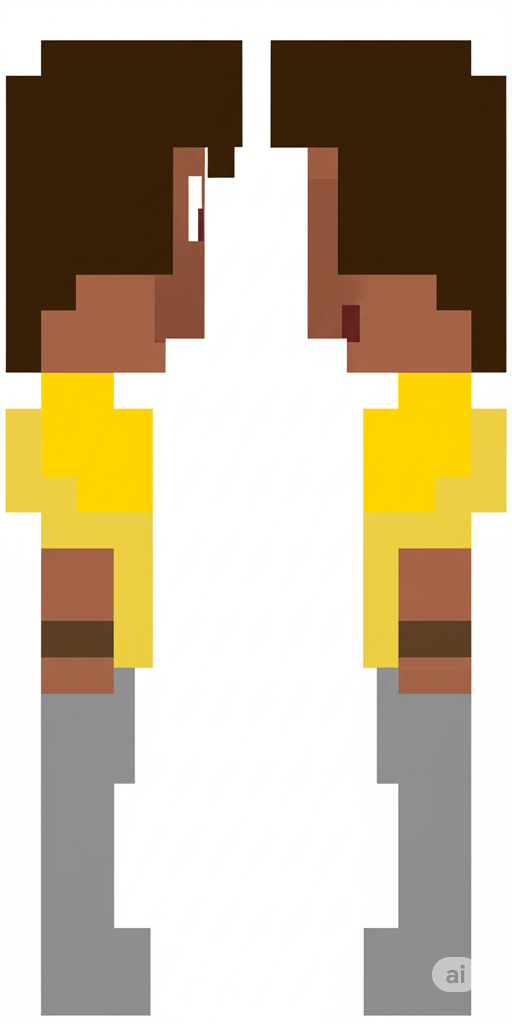
\includegraphics[width=0.5\linewidth]{figs/geminiPro/chat1/res1_tela1.png}
        \legend{\small Fonte: Elaborada pela autora, utilizando a ferramenta Gemini Pro.}
    \end{minipage}\hfill
    \begin{minipage}{0.45\textwidth}
        \centering
        \caption{\small Melhor sprite em side view gerado nos testes iniciais no Gemini Pro}
        \label{fig:GeminiProSpriteSideMelhor1}
        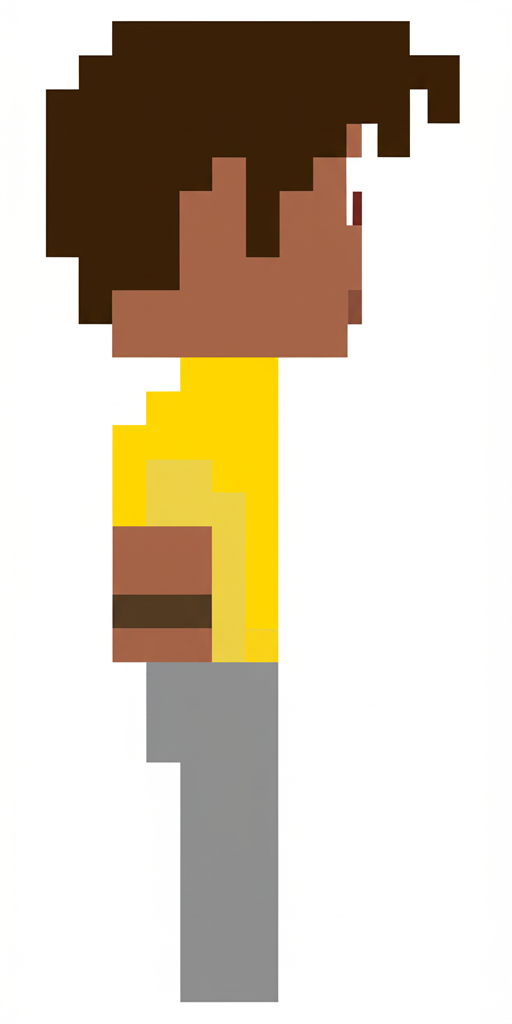
\includegraphics[width=0.5\linewidth]{figs/geminiPro/chat1/res4_tela1.png}
        \legend{\small Fonte: Elaborada pela autora, utilizando a ferramenta Gemini Pro.}
    \end{minipage}
\end{figure}

Como as deformações mais chamativas estavam na região da cabeça, nos testes posteriores (Figura \ref{fig:geminiPro2}) foram anexadas as Figuras \ref{fig:geminiProPabloChatGPTSide} e \ref{fig:geminiProPabloPixelLab} (até aquele momento, os melhores sprites em side view gerados, respectivamente, pelo ChatGPT e pelo Pixel Lab) para auxiliar especificamente na geração da cabeça. O resultado (Figura \ref{fig:GeminiProSpriteCorpoErrado}) apresentou a cabeça menos deformada, porém apresentou o mesmo erro de formato no corpo que uma das imagens anexadas possuía, além de copiar o fundo com quadrados cinzas dela.

\begin{figure}[htbp]
    \centering
    \caption{\small Sprite gerado em side view com o formato de corpo errado no Gemini Pro}
    \label{fig:GeminiProSpriteCorpoErrado}
    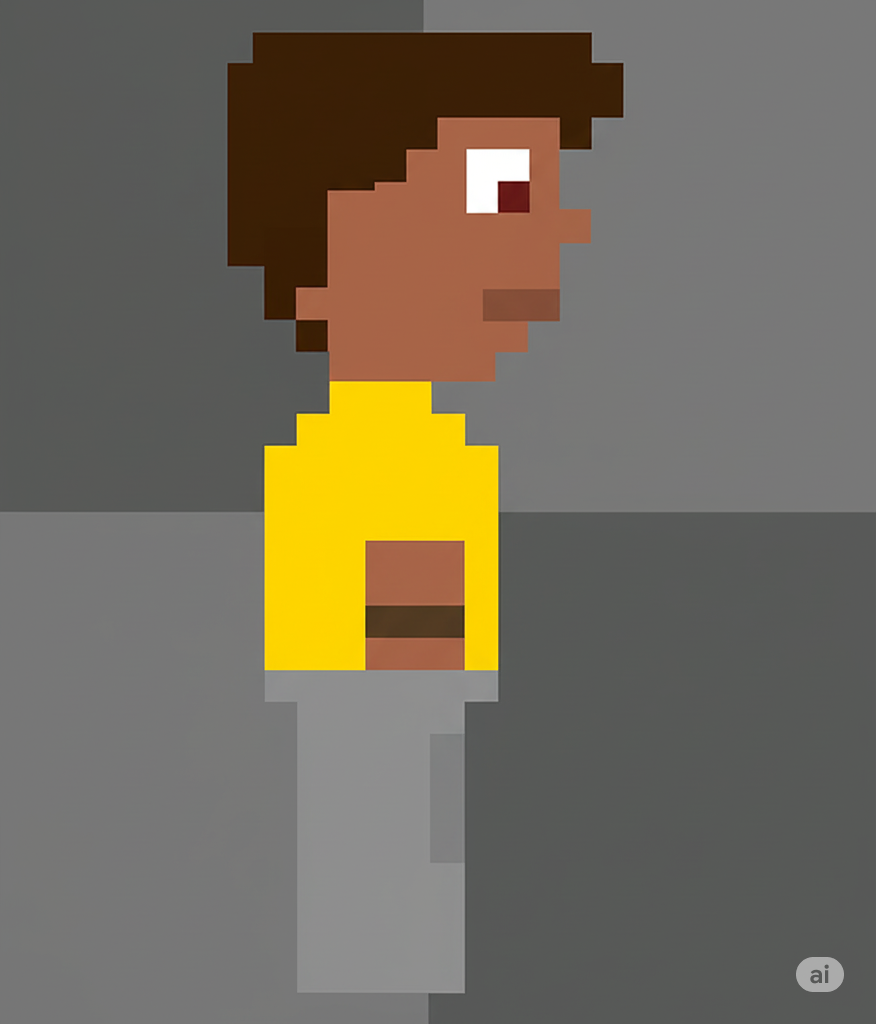
\includegraphics[width=0.2\linewidth]{figs/geminiPro/chat1/res1_tela2.png}
    \legend{\small Fonte: Elaborada pela autora, utilizando a ferramenta Gemini Pro.}
\end{figure}

No prompt seguinte, a IA foi instruída a manter a cabeça da Figura \ref{fig:GeminiProSpriteCorpoErrado} e o corpo da Figura \ref{fig:GeminiProSpriteSideMelhor1}, porém a ferramenta não gerou um resultado preciso e ainda manteve o fundo quadriculado, como pode ser visto na Figura \ref{fig:GeminiProSpriteFundoCopia}. O teste completo pode ser consultado na Figura \ref{fig:geminiPro3} no Apêndice \ref{ap.telasIA}.

\begin{figure}[htbp]
    \centering
    \caption{\small Sprite gerado em side view com o fundo quadriculado}
    \label{fig:GeminiProSpriteFundoCopia}
    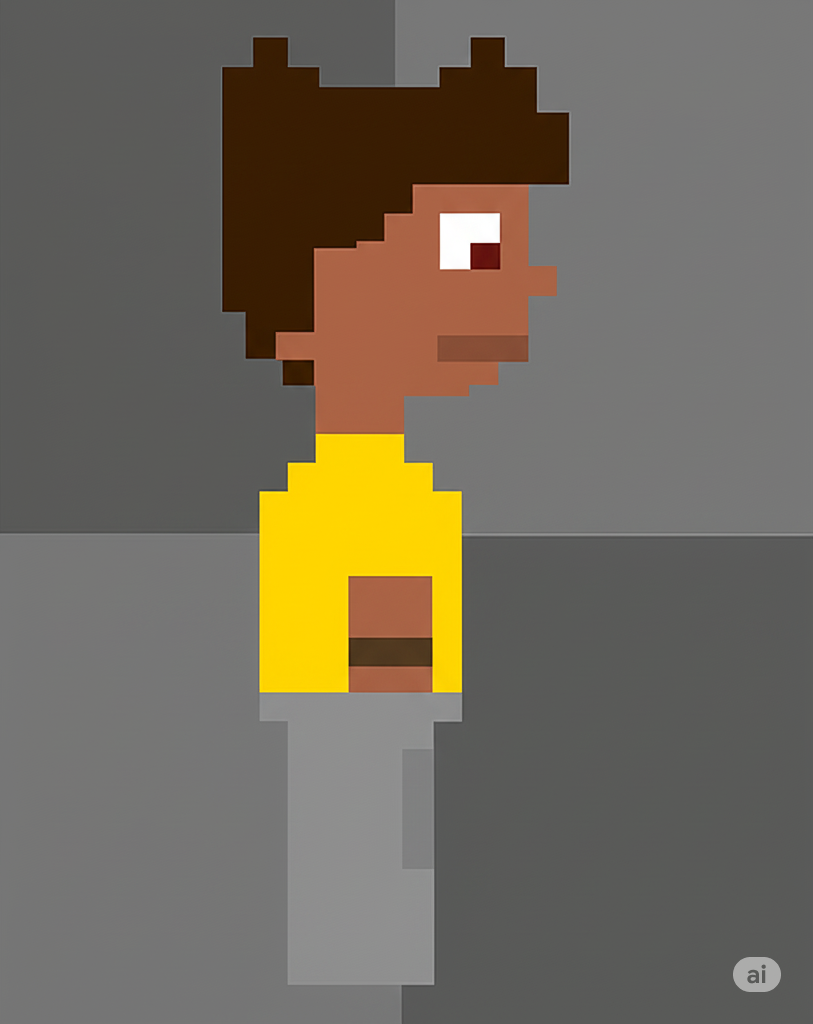
\includegraphics[width=0.2\linewidth]{figs/geminiPro/chat1/res1_tela3.png}
    \legend{\small Fonte: Elaborada pela autora, utilizando a ferramenta Gemini Pro.}
\end{figure}

Como a imagem do Pixel Lab estava claramente afetando mais do que o esperado os resultados, foi criado um novo chat para novamente gerar imagens sem essa influência no contexto da IA. Foi anexado o sprite em front view e escrito o prompt para rotacionar o personagem. Os resultados gerados foram satisfatórios, apresentando uma performance bem melhor em relação ao primeiro teste, apesar dos prompts serem quase idênticos, como pode ser visto nas Figuras \ref{fig:geminiProSideComparaPrompt} e \ref{fig:geminiProSideComparaMelhor}. Vale destacar que visivelmente nenhum resultado apresentou o padrão pixel perfect. A interação pode ser vista na Figura \ref{fig:geminiPro4} no Apêndice \ref{ap.telasIA}.

\begin{figure}[htbp]
    \centering
    \caption{\small Comparação dos prompts utilizados para geração do sprite em side view usando apenas o front view de referência no Gemini Pro}
    \label{fig:geminiProSideComparaPrompt}
    \begin{subfigure}{0.45\linewidth}
        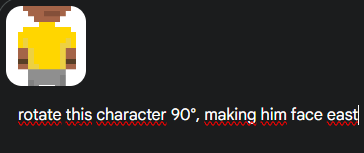
\includegraphics[width=1\linewidth]{figs/geminiPro/chat1/prompt.PNG}
        \caption{\small Prompt utilizado nas gerações com o rosto deformado}
        \label{fig:geminiProSideCompararPrompt1}
    \end{subfigure}\hfill
    \begin{subfigure}{0.45 \linewidth}
        \centering
        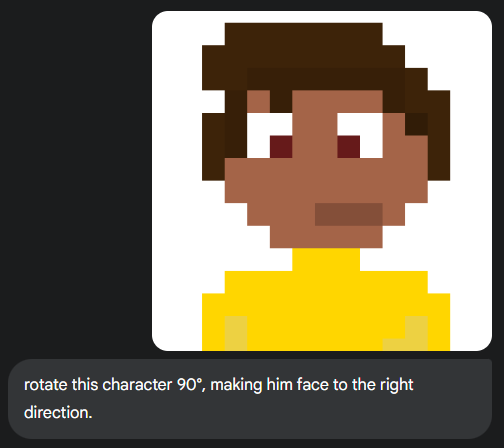
\includegraphics[width=1\linewidth]{figs/geminiPro/chat2/prompt.PNG}
        \caption{\small Prompt utilizado nas gerações satisfatórias}
        \label{fig:geminiProSideCompararPrompt2}
    \end{subfigure}
    \legend{\small Fonte: Elaborada pela autora.}
\end{figure}

\begin{figure}[htbp]
    \centering
    \caption{\small Comparação dos resultados em side view usando apenas o front view de referência no Gemini Pro}
    \label{fig:geminiProSideComparaMelhor}
    \begin{subfigure}{0.45\linewidth}
        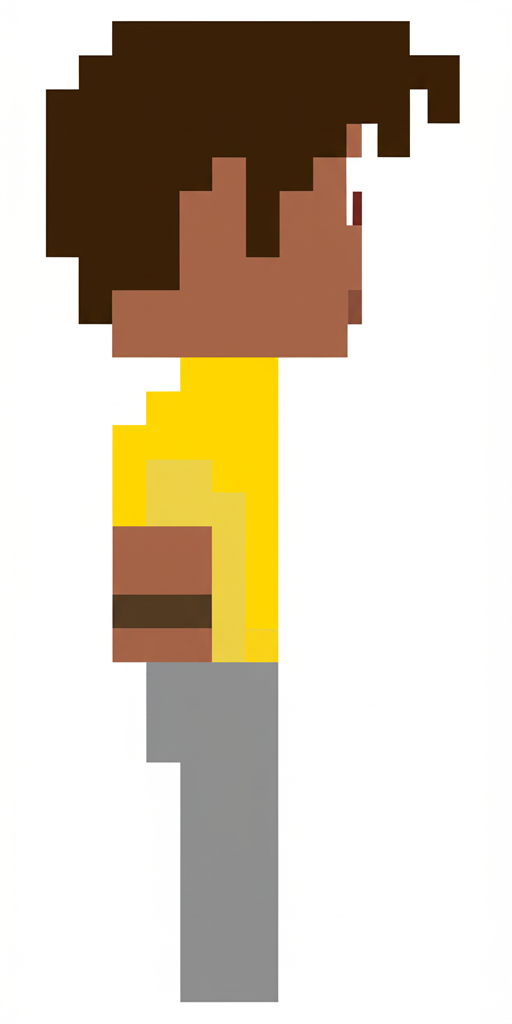
\includegraphics[width=0.7\linewidth]{figs/geminiPro/chat1/res4_tela1.png}
        \caption{\small Melhor resultado do teste inicial no primeiro chat}
        \label{fig:geminiProSideCompararMelhor1}
    \end{subfigure}\hfill
    \begin{subfigure}{0.45 \linewidth}
        \centering
        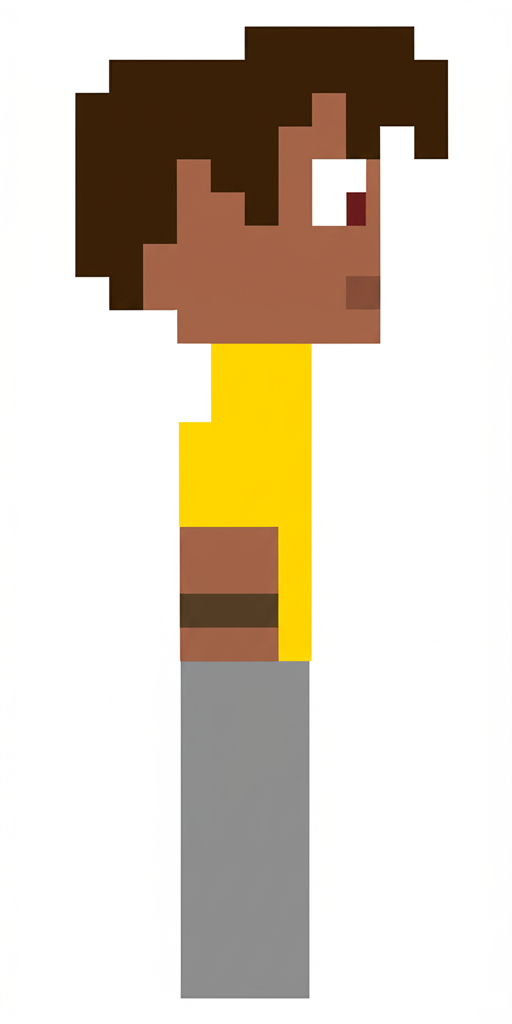
\includegraphics[width=0.7\linewidth]{figs/geminiPro/chat2/res1_tela1.png}
        \caption{\small Melhor resultado do teste inicial no segundo chat}
        \label{fig:geminiProSideCompararMelhor2}
    \end{subfigure}
    \legend{\small Fonte: Elaborada pela autora.}
\end{figure}

Numa tentativa de verificar se a ferramenta era capaz de produzir um resultado ainda melhor, foi usada a Figura \ref{fig:geminiProSideCompararMelhor2} como referência de como as próximas rotações deveriam ficar. Os sprites gerados apresentaram uma performance pior, com erros na rotação e deformações no rosto. Essa interação é demonstrada na Figura \ref{fig:geminiPro5} no Apêndice \ref{ap.telasIA}.

Mais alguns testes foram feitos para entender quais mudanças no prompt e nos arquivos enviados poderiam aumentar ou diminuir a qualidade dos sprites gerados. 

Adicionar a descrição do personagem não trouxe nenhuma mudança significativa na qualidade dos resultados, gerando inclusive outros resultados satisfatórios, como pode ser visto na Figura \ref{fig:geminiProSideMelhorDescricao}. Os testes com a descrição adicionada ao prompt podem ser consultados nas Figuras \ref{fig:geminiPro6} a \ref{fig:geminiPro9}.

\begin{figure}[htbp]
    \centering
    \caption{\small Melhores resultados em side view adicionando a descrição do personagem no Gemini Pro}
    \label{fig:geminiProSideMelhorDescricao}
    \begin{subfigure}{0.45\linewidth}
        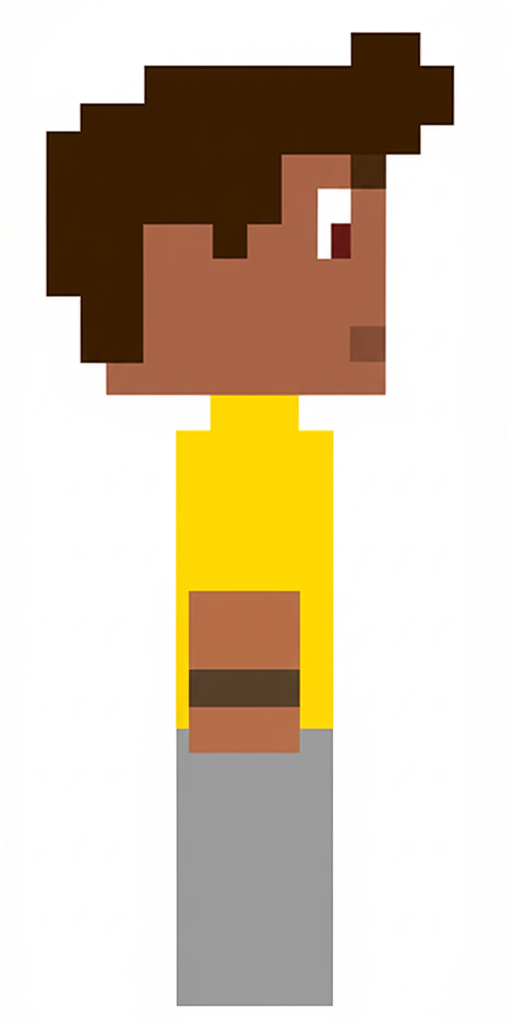
\includegraphics[width=0.7\linewidth]{figs/geminiPro/chat2/res1_tela3.png}
        \caption{\small Resultado 1}
        \label{fig:geminiProSideMelhorDescricao1}
    \end{subfigure}\hfill
    \begin{subfigure}{0.45 \linewidth}
        \centering
        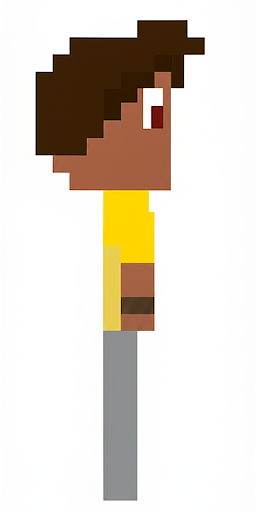
\includegraphics[width=0.7\linewidth]{figs/geminiPro/chat5/tela3_res2.PNG}
        \caption{\small Resultado 2}
        \label{fig:geminiProSideMelhorDescricao2}
    \end{subfigure}
    \legend{\small Fonte: Elaborada pela autora.}
\end{figure}

Escrever um prompt instruindo a ferramenta a fazer o sprite do personagem olhando para a direita e adicionar mais imagens de referências (Figuras \ref{fig:geminiProPablo} a \ref{fig:geminiProPabloPixelLab45_2}), dando o contexto do que cada figura representa em diferentes mensagens, fez com que a IA gerasse um sprite inconsistente com o estilo de pixel art (Figura \ref{fig:GeminiProInconsistenteMelhor}). Ao observar o raciocínio da IA (Figura \ref{fig:GeminiProRaciocinioGeracaoImagem}), foi descoberto que o Gemini apenas formula um prompt para ser enviado ao modelo especializado na geração de imagens, que na época era o Imagen 4. Com isso, foi levantada a hipótese de que, como os sprites de referência foram anexados numa mensagem anterior, o modelo de chat não estava passando essas figuras para o Imagen 4 na hora de gerar a imagem. Para confirmar isso, a ideia era comparar o raciocínio da geração consistente com a da inconsistente, porém em nenhuma das imagens consistentes havia a opção de mostrar os pensamentos. Dessa forma, não foi possível testar a validade da teoria. As Figuras \ref{fig:geminiPro10} a \ref{fig:geminiPro13} no Apêndice \ref{ap.telasIA} demonstram esta bateria de testes.

\begin{figure}[htbp]
    \centering
    \caption{\small Melhor resultado em side view utilizando múltiplas imagens de referência e um contexto maior no Gemini Pro}
    \label{fig:GeminiProInconsistenteMelhor}
    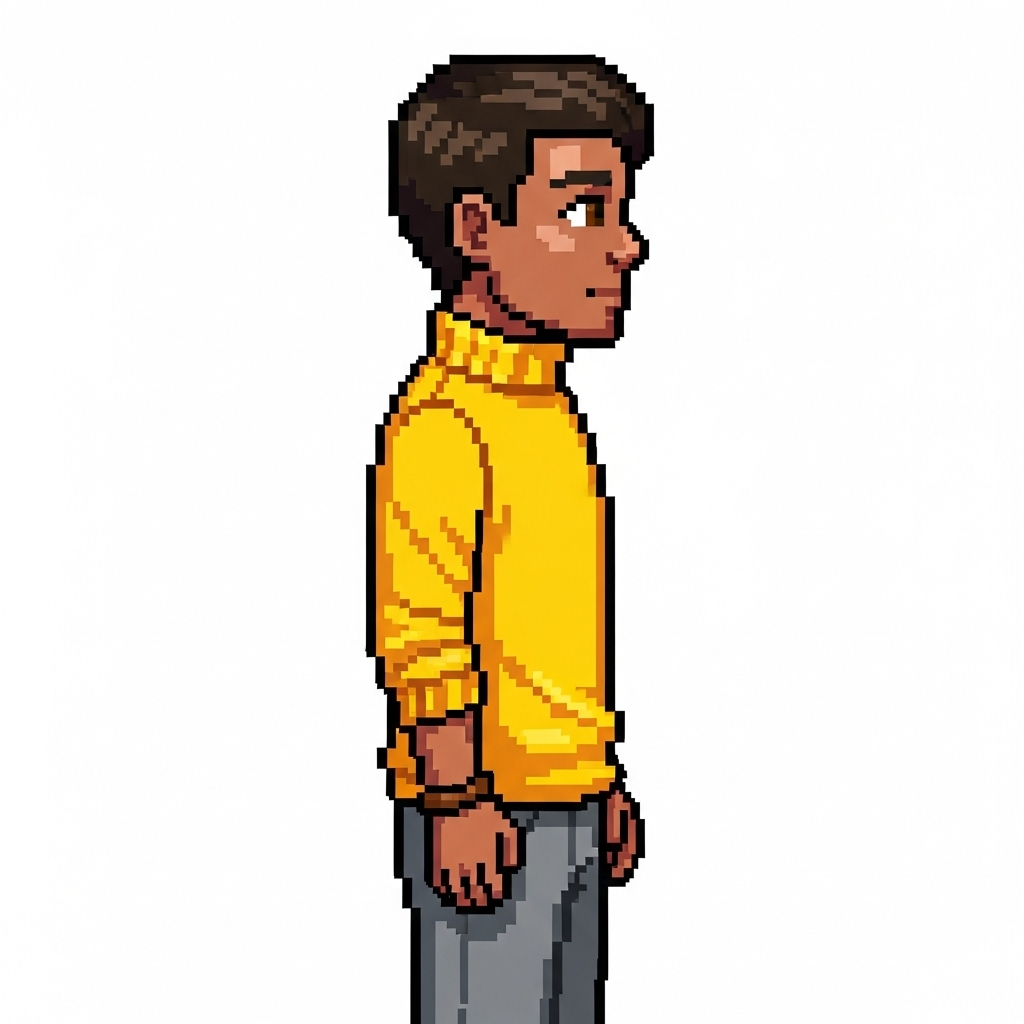
\includegraphics[width=0.2\linewidth]{figs/geminiPro/chat4/res1_tela16.png}
    \legend{\small Fonte: Elaborada pela autora, utilizando a ferramenta Gemini Pro.}
\end{figure}

\begin{figure}[htbp]
    \centering
    \caption{\small Raciocínio do Gemini Pro antes de gerar a imagem}
    \label{fig:GeminiProRaciocinioGeracaoImagem}
    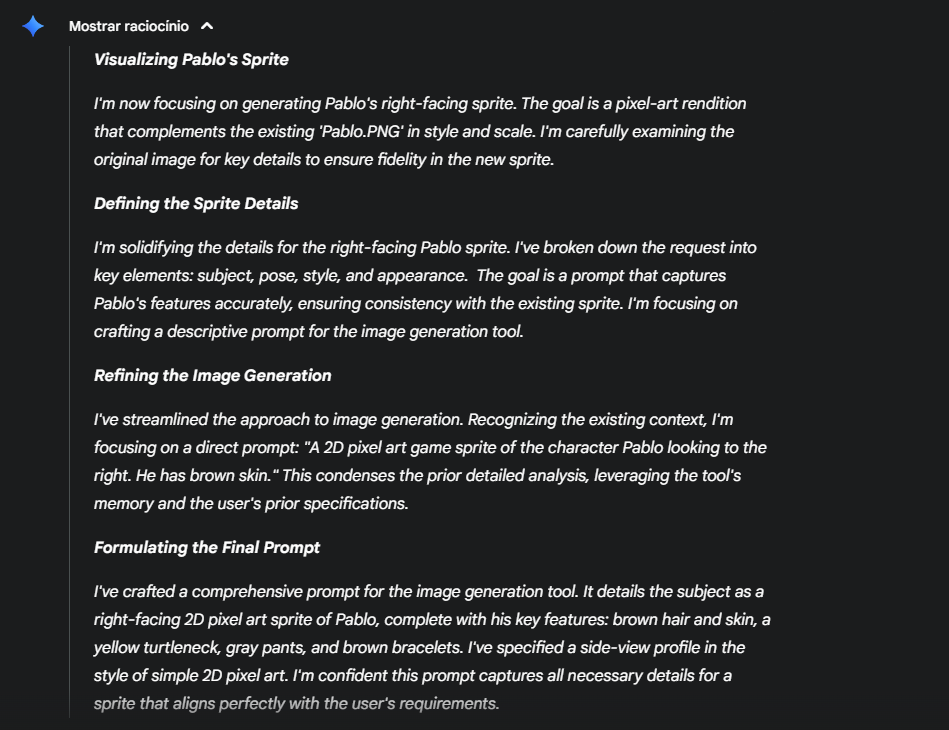
\includegraphics[width=0.8\linewidth]{figs/geminiPro/chat4/tela5.PNG}
    \legend{\small Fonte: Elaborada pela autora.}
\end{figure}

Utilizar como referência o sprite rotacionado em 45 graus (Figura \ref{fig:geminiProPabloPixelLab45_2}), com o prompt pedindo uma rotação de 45 graus para o personagem ficar em side view, gerou o personagem na visão incorreta, como pode ser visto na Figura \ref{fig:GeminiPro45Melhor}. Essa interação pode ser verificada nas Figuras \ref{fig:geminiPro14} a \ref{fig:geminiPro16} no Apêndice \ref{ap.telasIA}.

\begin{figure}[htbp]
    \centering
    \caption{\small Resultado em side view utilizando o sprite rotacionado em 45 graus como referência no Gemini Pro}
    \label{fig:GeminiPro45Melhor}
    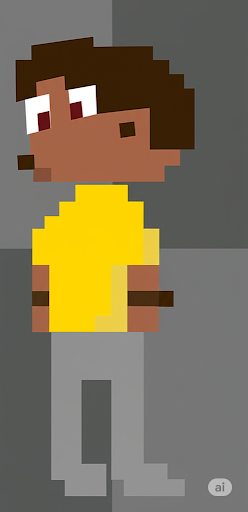
\includegraphics[width=0.2\linewidth]{figs/geminiPro/chat5/tela4_res2.png}
    \legend{\small Fonte: Elaborada pela autora, utilizando a ferramenta Gemini Pro.}
\end{figure}

Foi feita uma última tentativa em gerar um sprite ainda melhor do que o anteriormente gerado, focando em redesenhar o personagem utilizando as imagens dele em side view como referência (Figuras \ref{fig:geminiProPabloPixelLab} e \ref{fig:geminiProSideCompararMelhor2}) em vez de realizar a rotação. A ideia era manter a cabeça parecida com a do melhor sprite em side view gerado pelo Gemini Pro até o momento, e manter o corpo com relevo em ambos os lados, como acontecia no melhor sprite em side view gerado pelo Pixel Lab. O resultado gerado inicialmente foi editado na própria ferramenta através de outros prompts, formando a Figura \ref{fig:GeminiProSideMelhor}. O processo completo pode ser consultado nas Figuras \ref{fig:geminiPro17} a \ref{fig:geminiPro19} no Apêndice \ref{ap.telasIA}.

\begin{figure}[htbp]
    \centering
    \caption{\small Melhor resultado em side view gerado pelo Gemini Pro}
    \label{fig:GeminiProSideMelhor}
    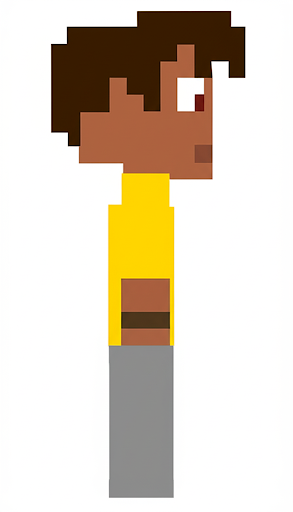
\includegraphics[width=0.3\linewidth]{figs/geminiPro/chat6/tela3_res1.png}
    \legend{\small Fonte: Elaborada pela autora, utilizando a ferramenta Gemini Pro.}
\end{figure}

Posteriormente, essa imagem foi passada para o padrão pixel perfect utilizando o Pixilart (mencionado anteriormente). Ainda dentro do Pixilart, foram feitos pequenos ajustes para corrigir os erros gerados durante a conversão. Esse processo pode ser verificado na Figura \ref{fig:geminiProSideEdicaoMelhor}. Por último, o sprite foi exportado para a ferramenta Pixel Lab, onde mais ajustes foram realizados (detalhados na Seção \ref{s.pixelLab}).

\begin{figure}[htbp]
    \centering
    \caption{\small Processo de edição do melhor sprite em side view no Pixilart}
    \label{fig:geminiProSideEdicaoMelhor}
    \begin{subfigure}{0.32\linewidth}
        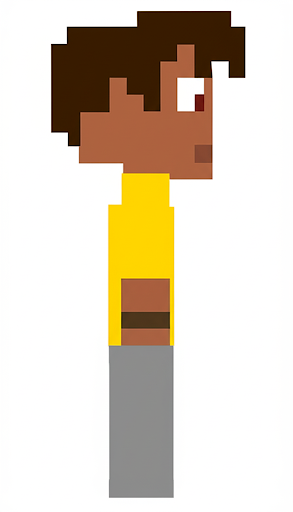
\includegraphics[width=1\linewidth]{figs/geminiPro/chat6/tela3_res1.png}
        \caption{\small Melhor sprite em side view gerado pelo Gemini Pro antes de converter para pixel perfect}
        \label{fig:geminiProSideEdicaoMelhorAntesEdicao}
    \end{subfigure}\hfill
    \begin{subfigure}{0.32\linewidth}
        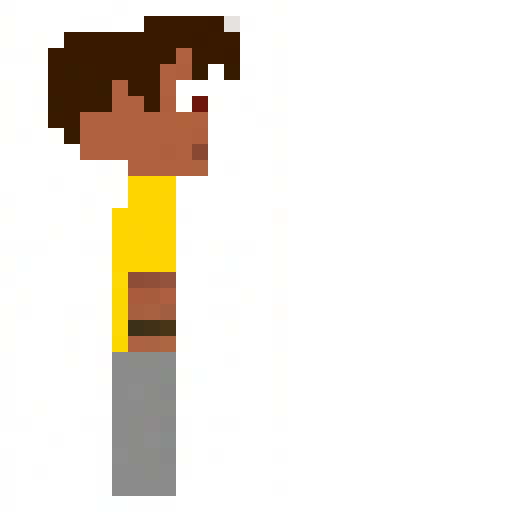
\includegraphics[width=1\linewidth]{figs/geminiPro/passa_pixel_grande.png}
        \caption{\small Sprite em side view após conversão para pixels no Pixilart}
        \label{fig:geminiProSideEdicaoMelhorAposConversao}
    \end{subfigure}\hfill
    \begin{subfigure}{0.32 \linewidth}
        \centering
        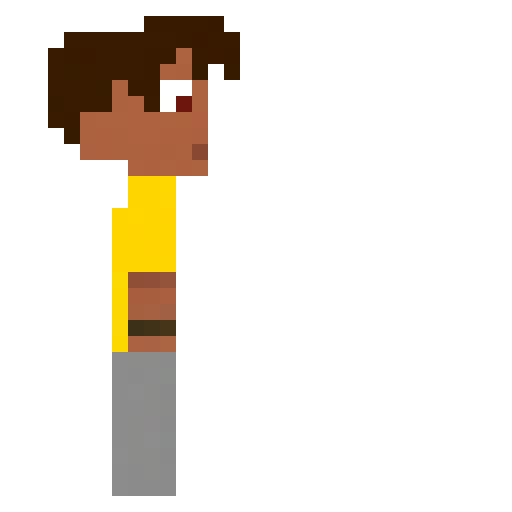
\includegraphics[width=1\linewidth]{figs/geminiPro/fix grande.png}
        \caption{\small Sprite em side view após edição no Pixilart}
        \label{fig:geminiProSideEdicaoMelhorAposEdicao}
    \end{subfigure}
    \legend{\small Fonte: Elaborada pela autora.}
\end{figure}

Conclui-se que o Gemini Pro demonstrou um desempenho superior em relação às ferramentas anteriores na geração do sprite em side view, mantendo alta consistência com o personagem e o estilo em quase todos os testes e sendo preciso na interpretação dos prompts na maioria dos casos. Apesar disso, os resultados não possuem o padrão pixel perfect e a eficácia da IA é sensível ao contexto da conversa, o que pode exigir a criação de novos chats para evitar uma repetição de erros. Embora a edição de imagens diretamente na plataforma seja limitada ao uso da IA, a capacidade dessa ferramenta em gerar um desenho base coeso e de alta qualidade solidifica seu papel na eficiência na produção de poses para auxílio no processo de animação.

